\documentclass{article}
%\usepackage[brazil]{babel}
\usepackage[utf8]{inputenc}
\usepackage{geometry}
\usepackage{tikz}
\usepackage{amsmath}
\usepackage{amssymb}
\usetikzlibrary{arrows.meta,
                chains,
                fit,
                positioning,
                quotes}

\begin{document}
	\begin{center}
	\section*{\normalsize  Catálogo Gaia de estrelas até $23.0$ parsecs do Sol\\}
	\end{center}
	\vspace{50pt}

\begin{enumerate}
	\item A interseção aumentou de $744$ para $755$ ($11$ estrelas a mais).
	\item Como está sendo feita a interseção:\\
	Fixada uma designação Gaia, é buscado no Simbad todos os identificadores para esta designação. Os identificadores para a estrela HD $146233$ são os seguintes:
	
	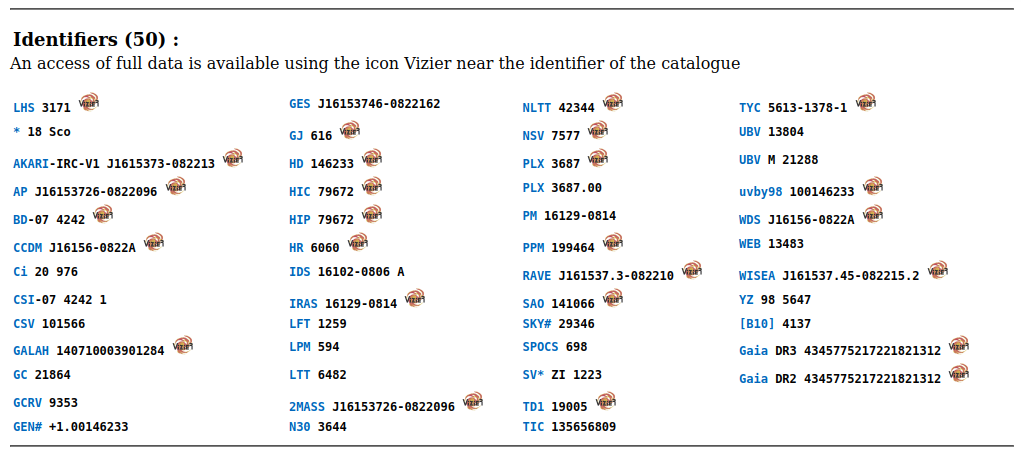
\includegraphics[scale=0.35]{identifiers.png}
	
	Depois, selecionamos somente os identificadores que começam por HIP, se houver algum. O identificador é anexado no registro da estrela Gaia. 
	
	\item Gaia $\cap$ Hipparcos: No diagrama $M(Vt)$ versus $BT-VT$, saíram $2$ estrelas. Passou de $556$ estrelas para $554$ estrelas.
	
	\item Hipparcos $-$ Gaia: No diagrama $M(Vt)$ versus $BT-VT$, saíram $2$ estrelas. Passou de $635$ estrelas para $633$ estrelas. 
	
	\item No Diagrama Hipparcos $-$ Gaia,  $M(V)$  versus $B-V$, tem uma estrela no canto inferior direito que não estava aparecendo no diagrama anterior porque o tamanho da imagem estava pequeno
	
	\item Somando-se as estrelas não plotadas com as plotadas, obtemos o total de estrelas do sub catálogo
	
	\item No botão Gaia $-$ Hipparcos, a estrela que está em vermelho no diagrama $M(G)$ versus $Bp-Rp$ é a HD $131156$B
	
	\item A estrela que aparece em azul nos diagramas é a HD $146233$.
\end{enumerate}

\newpage

\begin{equation*}
	\begin{aligned}
		M(G) &= phot\_g\_mean\_mag + 5 + 5 \cdot \log_{10}\bigg(\frac{parallax}{1000}\bigg)\\[15pt]
		M(G)^{+} &= phot\_g\_mean\_mag + 5 + 5 \cdot \log_{10}\bigg(\frac{parallax + parallax\_error}{1000}\bigg)\\[15pt]
		M(G)^{-} &= phot\_g\_mean\_mag + 5 + 5 \cdot \log_{10}\bigg(\frac{parallax - parallax\_error}{1000}\bigg)\\[15pt]
		M(G) \; error & = \frac{\mid M(G) - M(G)^{+} \mid + \mid M(G) - M(G)^{-} \mid}{2}\\[15pt]
		B_p - R_p & = phot\_pb\_mean\_mag - phot\_rp\_mean\_mag
	\end{aligned}
\end{equation*}

\vspace{50pt}

\begin{equation*}
	\begin{aligned}
		M(R_p) &= phot\_rp\_mean\_mag + 5 + 5 \cdot \log_{10}\bigg(\frac{parallax}{1000}\bigg)\\[15pt]
		M(R_p)^{+} &= phot\_rp\_mean\_mag + 5 + 5 \cdot \log_{10}\bigg(\frac{parallax + parallax\_error}{1000}\bigg)\\[15pt]
		M(R_p)^{-} &= phot\_rp\_mean\_mag + 5 + 5 \cdot \log_{10}\bigg(\frac{parallax - parallax\_error}{1000}\bigg)\\[15pt]
		M(R_p) \; error & = \frac{\mid M(R_p) - M(R_p)^{+} \mid + \mid M(R_p) - M(R_p)^{-} \mid}{2}\\[15pt]
		B_p - R_p & = phot\_pb\_mean\_mag - phot\_rp\_mean\_mag
	\end{aligned}
\end{equation*}

\newpage

\begin{equation*}
	\begin{aligned}
		M(V) &= V_{mag} + 5 + 5 \cdot \log_{10}\bigg(\frac{Plx}{1000}\bigg)\\[15pt]
		M(V)^{+} &= V_{mag} + 5 + 5 \cdot \log_{10}\bigg(\frac{Plx + e\_Plx}{1000}\bigg)\\[15pt]
		M(V)^{-} &= V_{mag} + 5 + 5 \cdot \log_{10}\bigg(\frac{Plx - e\_Plx}{1000}\bigg)\\[15pt]
		M(V) \; error & = \frac{\mid M(V) - M(V)^{+} \mid + \mid M(V) - M(V)^{-} \mid}{2}\\[15pt]
	\end{aligned}
\end{equation*}

\vspace{50pt}

\begin{equation*}
	\begin{aligned}
		M(V_t) &= VT_{mag} + 5 + 5 \cdot \log_{10}\bigg(\frac{Plx}{1000}\bigg)\\[15pt]
		M(V_t)^{+} &= VT_{mag} + 5 + 5 \cdot \log_{10}\bigg(\frac{Plx + e\_Plx}{1000}\bigg)\\[15pt]
		M(V_t)^{-} &= VT_{mag} + 5 + 5 \cdot \log_{10}\bigg(\frac{Plx - e\_Plx}{1000}\bigg)\\[15pt]
		M(V_t) \; error & = \frac{\mid M(V_t) - M(V_t)^{+} \mid + \mid M(V_t) - M(V_t)^{-} \mid}{2}\\[15pt]
		BT - VT &= BT_{mag} - VT_{mag}
	\end{aligned}
\end{equation*}

\newpage

\end{document}